\section{}
The aluminum rectangular parallelepiped ($E$ = 70 GPa and $\nu = \frac{1}{3}$) shown in Fig. \ref{fig:Q2} has dimensions 
$a = \qty{150}{mm}$, $b = \qty{100}{mm}$, and $c = \qty{75}{mm}$. It is subjected to tri-axial stresses 
$\sigma_x = \qty{70}{MPa}$, $\sigma_y = \qty{-30}{MPa}$, and $\sigma_z = \qty{-15}{MPa}$ acting on the 
$x$, $y$, and $z$ faces, respectively. Determine,

\begin{figure}[h]
    \centering
    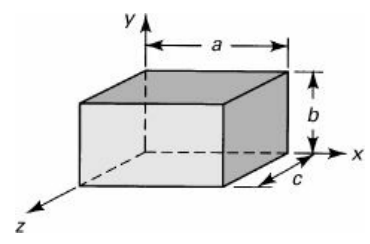
\includegraphics[width=0.5\linewidth]{Questions/Figures/Q2ProblemDiagram.png}
    \caption{Rectangular parallelepiped subjected to tri-axial stresses.}
    \label{fig:Q2}
\end{figure}

\begin{enumerate}[label=(\alph*)]
    \item the changes $\Delta a$, $\Delta b$, and $\Delta c$ in the dimensions of the block.
    \item the change $\Delta V$ in the volume.
\end{enumerate}


\textbf{Solution}
\subsection{}
From the generalized Hooke's law, the stress-strain relation is given by:
\[
\begin{aligned}
    \epsilon_x &= \frac{1}{E} (\sigma_x - \nu(\sigma_y + \sigma_z)) \\
    \epsilon_y &= \frac{1}{E} (\sigma_y - \nu(\sigma_x + \sigma_z)) \\
    \epsilon_z &= \frac{1}{E} (\sigma_z - \nu(\sigma_x + \sigma_y)) \\
\end{aligned}
\]

From the definition of strain,
\[
\begin{aligned}
    \Delta x &= \epsilon_x a \\
    \Delta y &= \epsilon_y b \\
    \Delta z &= \epsilon_z c \\
\end{aligned}
\]

By direct substitution,
\[
\begin{aligned}
    \Delta x &= \frac{1}{E} (\sigma_x - \nu(\sigma_y + \sigma_z)) a \\
    &= \frac{1}{70\times 10^3} (70 - \frac{1}{3}(-30 - 15)) 150 \\
    &= \boxed{\qty{0.182}{mm}} \\
    \Delta b &= \frac{1}{E} (\sigma_y - \nu(\sigma_x + \sigma_z)) b \\
    &= \frac{1}{70\times 10^3} (-30 - \frac{1}{3}(70 - 15)) 100 \\
    &= \boxed{\qty{-0.0690}{mm}} \\
    \Delta c &= \frac{1}{E} (\sigma_z - \nu(\sigma_x + \sigma_y)) c \\
    &= \frac{1}{70\times 10^3} (-15 - \frac{1}{3}(70 - 30)) 75 \\
    &= \boxed{\qty{-0.0304}{mm}} \\
\end{aligned}
\]

\subsection{}
The change in volume is given by:
\[
\begin{aligned}
    \Delta V &= e V_0 \\
\end{aligned}
\]

Where dilation $e$ is given by:
\[
\begin{aligned}
    e = \epsilon_x + \epsilon_y + \epsilon_z = &= \frac{1-2 \nu}{E} (\sigma_x + \sigma_y + \sigma_z) \\
    &= \frac{1- \frac{2}{3}}{70\times 10^3} (70 - 30 - 15) \\
    &= \qty{1.1905e-4}{}
\end{aligned}
\]

Therefore,
\[
\begin{aligned}
    \Delta V &= e V_0 \\
    &= (1.1905 \times 10^{-4})(150)(100)(75) \\
    &= \boxed{\qty{134}{mm^3}}
\end{aligned}
\]